\begin{figure}
\centering
    \begin{subfigure}{0.48\linewidth}
        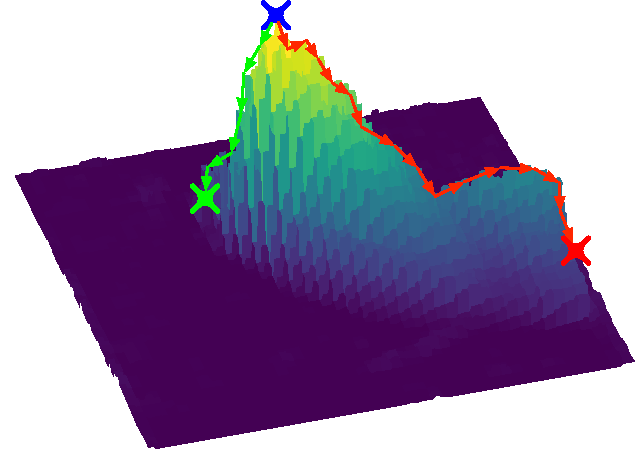
\includegraphics[width=\linewidth]{./img/scene_learning/ridge_climbing.pdf}
        \subcaption{}
        \label{subfig:scene-ridge-climbing}
    \end{subfigure}
    \begin{subfigure}{0.48\linewidth}
        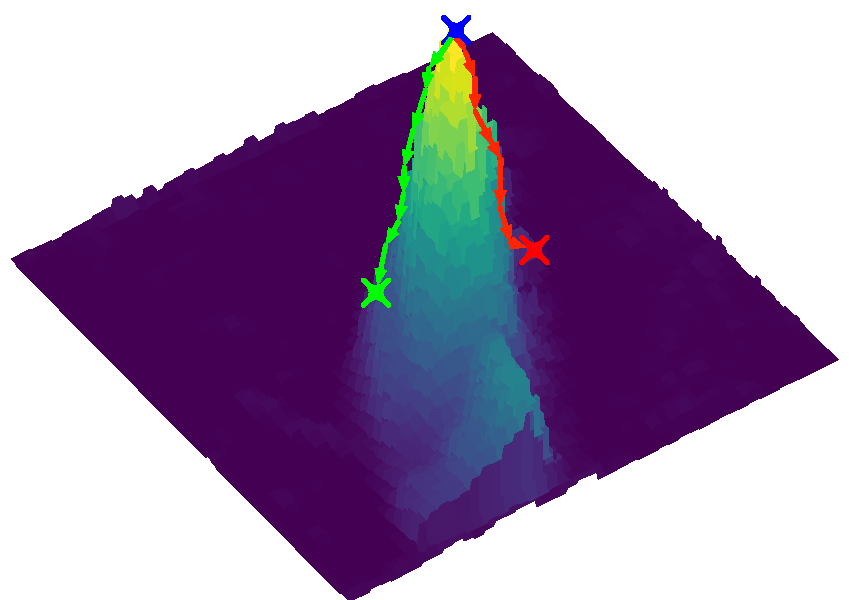
\includegraphics[width=\linewidth]{./img/scene_learning/ridge_climbing_perp.pdf}
        \subcaption{}
        \label{subfig:scene-ridge-climbing-perp}
    \end{subfigure}%
    \caption{Ridge climbing methods on a topic distribution: along the most likely topic direction (a) and its perpendicular direction (b). Blue cross indicates the starting point, red and green point indicates the end point.}
    \label{fig:scene-ridge-clibming}
\end{figure}